\chapter{Experimental Setup}\label{cha:setup}

\section{The Large Hadron Collider}\label{sec:setup:lhc}

The Large Hadron Collider (LHC)~\cite{LHC} is currently the worlds largest and most powerful proton and heavy ion accelerator.
It is located at CERN (Conseil Européen pour la Recherche Nucléaire) near Geneva.

The LHC was constructed between 1998 and 2008 inside the circular, \unit[27]{km} long tunnel
of the former Large Electron--Positron (LEP) Collider, which shut down in 2000.
The tunnel is located between 50 and 175 meters below ground level and crossing the France--Switzerland border.
Both protons and heavy ions can be accelerated in two beam pipes in opposite direction.
In proton--proton collisions both beams can contain up to 2808 bunches which contain $10^{11}$ protons each.
The time distance between the bunches is \unit[25]{ns}.
To bend the proton beams 1232 superconducting dipole magnets are used, which can generate a magnetic field of up
to \unit[8.3]{T}.
Additional 392 quadrupole magnets are used to focus the beams.

The beams are collided at four \emph{interaction points} (IP), where the four major experiments ATLAS, CMS, LHCb, and ALICE
are located.
ATLAS and CMS are multipurpose detectors and are used to perform a wide range of measurements and searches.
The focus of LHCb are interactions of B-hadrons.
ALICE is specialized for measurements of heavy-ion collisions.
\cref{fig:setup:accelerators} shows a schematic overview of the LHC and its experiments.
The ATLAS experiment is discussed in detail in \cref{sec:setup:atlas}.
\begin{figure}[htb]
    \centering
    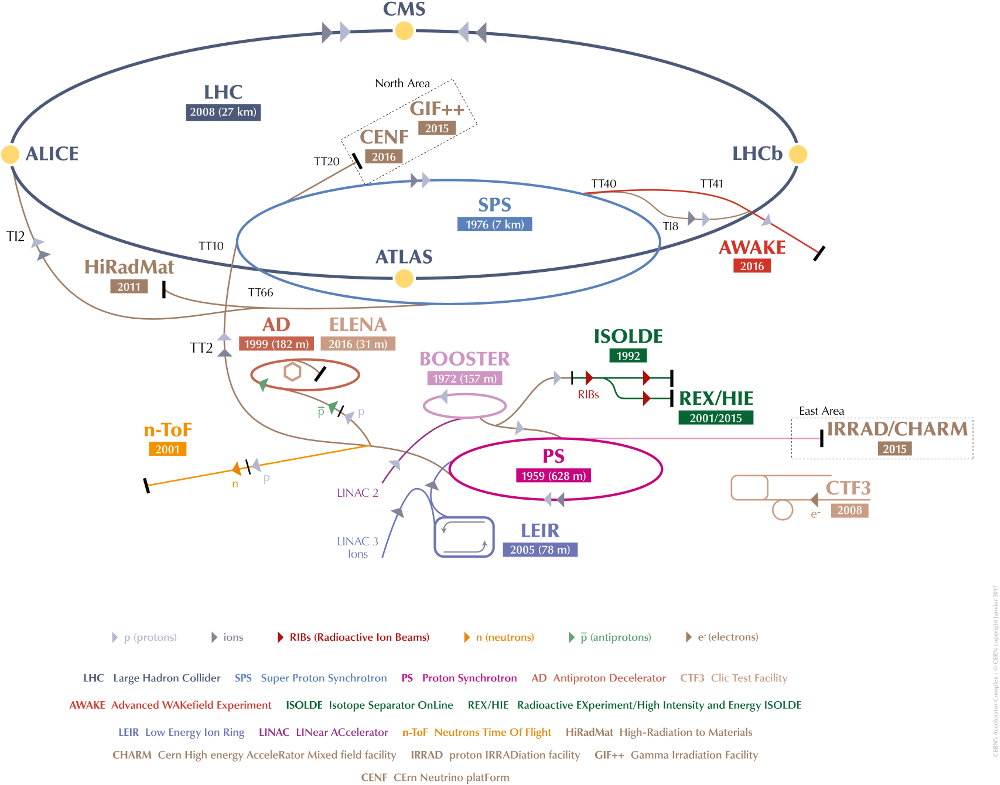
\includegraphics[width=0.9\textwidth]{./figures/setup/accelerators.png}
    \caption{The CERN accelerator complex, including the LHC and its preaccelerators.
             The four main experiments (ATLAS, CMS, LHCb, ALICE) are shown as a yellow dot.~\cite{Mobs:2197559}}\label{fig:setup:accelerators}
\end{figure}

The number of events per second which are generated in LHC collisions is given by
\begin{equation}
    N_\text{event} = \lumi \sigma_\text{event} \,,
\end{equation}
where $\sigma_\text{event}$ is the cross-section of the event and $\lumi$ the instantaneous luminosity.
The instantaneous luminosity is a quantity of the LHC and depends only the parameters of the beams.
For bunches with a Gaussian shape distribution it can be written as~\cite{LHC}
\begin{equation}
    \lumi = \frac{N_b^2 n_b f_\text{ref} \gamma_r}{4 \pi \epsilon_n \beta^*} F \,,
\end{equation}
where $N_b$ is the number of particles in each bunch, $n_b$ the number of bunches per beam, $f_\text{ref}$ the revolution
frequency of the particles, $\gamma_r$ the relativistic gamma factor, $\epsilon_n$ the normalized transverse beam emittance,
$\beta^*$ the beta function at the collision point, and $F$ the geometric luminosity reduction factor
due to the crossing angle of the beam at the interaction point.
The LHC is designed to collide protons with an instantaneous luminosity of up to $\lumi = \unit[10^{34}]{cm^2 s^{-1}}$
and a beam energy of up to \unit[7]{TeV}, which results in a collision with a center-of-mass energy of
$\sqrt{s} = \unit[14]{GeV}$.
Due to the high center-of-mass energies several preaccelerators which are shown in \cref{fig:setup:accelerators}
are needed to accelerate the particles to the desired velocity.

The previous and current data-taking periods and conditions of the LHC and ATLAS experiment are discussed in \cref{sec:setup:data}.

\section{The ATLAS Experiment}\label{sec:setup:atlas}

\subsection{Nomenclature}\label{sub:setup:nomenclature}

\subsection{Inner Detector}\label{sub:setup:id}

\subsection{Calorimeters}\label{sub:setup:calorimeters}

\subsection{Muon Spectrometer}\label{sub:setup:muons}

\subsection{Trigger System}\label{sub:setup:trigger}

\section{Data taking}\label{sec:setup:data}
